
\providecommand{\Cat}{\mathcal{C}at}

\section{绝对绝对提升图}\label{sec:absolute-absolute-lifting-diagrams}

回忆第 2 章中的\cref{def:absolute-left-lifting}：对 2-\trCategory{}中任意%
\trCospan{} $c\xrightarrow{g}a\xleftarrow{f}b$，$g$ 沿 $f$ 的一个%
\textbf{绝对右\trLifting}由
一支 1-\trCell{} $r$ 与一个 2-\trCell{} $\rho$ 给出，如下左图所示：
\begin{center}
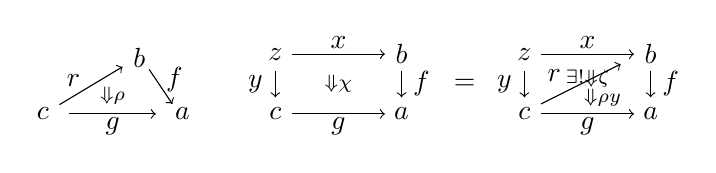
\begin{tikzpicture}[x=1.2em,y=1.2em]
  \node (c1) at (0,0) {$c$};
  \node (a1) at (4.2,0) {$a$};
  \node (b1) at (2.9,1.7) {$b$};
  \draw[->] (0.5,0.28) -- (2.4,1.42);
  \node at (0.92,1.02) {$r$};
  \draw[->] (3.2,1.34) -- (3.9,0.3);
  \node at (3.96,1.02) {$f$};
  \draw[->] (0.8,0) -- (3.4,0);
  \node at (2.1,-0.38) {$g$};
  \node at (2.1,0.55) {$\scriptstyle\Downarrow\rho$};
  \node (z2) at (7.0,1.8) {$z$};
  \node (b2) at (10.8,1.8) {$b$};
  \node (c2) at (7.0,0) {$c$};
  \node (a2) at (10.8,0) {$a$};
  \draw[->] (7.5,1.8) -- (10.3,1.8);
  \node at (8.9,2.14) {$x$};
  \draw[->] (10.8,1.3) -- (10.8,0.5);
  \node at (11.4,0.9) {$f$};
  \draw[->] (7.0,1.3) -- (7.0,0.5);
  \node at (6.4,0.9) {$y$};
  \draw[->] (7.5,0) -- (10.3,0);
  \node at (8.9,-0.38) {$g$};
  \node at (8.9,0.9) {$\scriptstyle\Downarrow\chi$};
  \node at (12.7,0.9) {$=$};
  \node (z3) at (14.5,1.8) {$z$};
  \node (b3) at (18.3,1.8) {$b$};
  \node (c3) at (14.5,0) {$c$};
  \node (a3) at (18.3,0) {$a$};
  \draw[->] (15.0,1.8) -- (17.8,1.8);
  \node at (16.4,2.14) {$x$};
  \draw[->] (18.3,1.3) -- (18.3,0.5);
  \node at (18.9,0.9) {$f$};
  \draw[->] (14.5,1.3) -- (14.5,0.5);
  \node at (13.9,0.9) {$y$};
  \draw[->] (15.0,0) -- (17.8,0);
  \node at (16.4,-0.38) {$g$};
  \draw[->] (15.0,0.3) -- (17.4,1.5);
  \node at (15.4,1.16) {$r$};
  \node at (16.4,1.05) {$\scriptstyle\exists!\Downarrow\zeta$};
  \node at (16.85,0.5) {$\scriptstyle\Downarrow\rho y$};
\end{tikzpicture}
\end{center}
从而，任何如中图所示的 2-\trCell{}都能唯一地经由 $(r,\rho)$ 分解成如右图所示的
形状。「绝对」这一形容词指的是如下性质：绝对右\trLifting{}图在沿任何
1-\trCell{} $k\colon d\to c$ 作限制下稳定。

下面这条引理给出第二重意义下为绝对的绝对右\trLifting{}图：亦即，它们被任何%
\trTwoFunctor{}保持。

\begin{lemma}\label{lem:absolute-lifting-under-adjunction}
设有\emph{在 $b$ 之下的}\trAdjunction{}（$f\dashv u$、$\eta\colon\mathrm{id}_{a}\Rightarrow uf$、
$\epsilon\colon fu\Rightarrow\mathrm{id}_{c}$），其意义如下：
\begin{itemize}
\item 涉及两个\trAdjunction{}的实箭头三角形均交换
\begin{center}
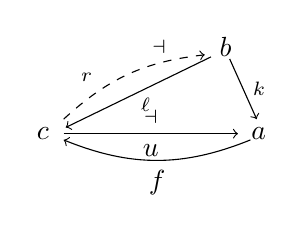
\begin{tikzpicture}[x=1.5em,y=1.5em]
  \node (b) at (4.4,2.1) {$b$};
  \node (c) at (0,0) {$c$};
  \node (a) at (5.2,0) {$a$};
  \draw[->,dashed] (0.5,0.35) to[bend left=18]
    node[pos=0.72,above]{$\scriptstyle\dashv$} (3.9,1.9);
  \node at (1.05,1.35) {$\scriptstyle r$};
  \draw[->] (4.05,1.85) -- node[below,pos=0.45]{$\scriptstyle\ell$} (0.55,0.15);
  \draw[->] (4.5,1.8) -- node[right,pos=0.5]{$\scriptstyle k$} (5.15,0.35);
  \draw[->] (0.5,0) -- (4.7,0);
  \node at (2.6,0.4) {$\scriptstyle\dashv$};
  \node at (2.6,-0.4) {$u$};
  \draw[->] (5.0,-0.15) to[bend left=22] node[below,pos=0.5]{$f$} (0.5,-0.15);
\end{tikzpicture}
\end{center}
\item 并且 $\eta k=\mathrm{id}_{k}$ 且 $\epsilon\ell=\mathrm{id}_{\ell}$。
\end{itemize}
此时，若 $\ell$ 容许一个\trRightAdjoint{} $r$，其\trUnit{}为
$\iota\colon\mathrm{id}_{b}\Rightarrow r\ell$、\trCounit{}为
$\nu\colon\ell r\Rightarrow\mathrm{id}_{c}$，则 $u\nu$ 展示 $r$ 为 $u$ 沿 $k$
的一个绝对右\trLifting{}：
\begin{center}
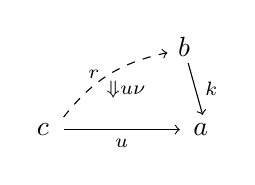
\begin{tikzpicture}[x=1.5em,y=1.5em]
  \node (b) at (3.4,2.0) {$b$};
  \node (c) at (0,0) {$c$};
  \node (a) at (3.8,0) {$a$};
  \draw[->,dashed] (0.5,0.3) to[bend left=20]
    node[left,pos=0.5]{$\scriptstyle r$} (3.0,1.85);
  \draw[->] (3.5,1.6) -- node[right]{$\scriptstyle k$} (3.85,0.35);
  \draw[->] (0.5,0) -- node[below]{$\scriptstyle u$} (3.3,0);
  \node at (2.0,0.95) {$\scriptstyle\Downarrow u\nu$};
\end{tikzpicture}
\end{center}
此外，这类绝对右\trLifting{}图被任何\trTwoFunctor{}保持。
\end{lemma}

\begin{proof}
论证是纯图解式的：任何如下左图所示的 2-\trCell{}都经由 $u\nu$ 分解，正如下图
链所展示的那样：
\begin{center}
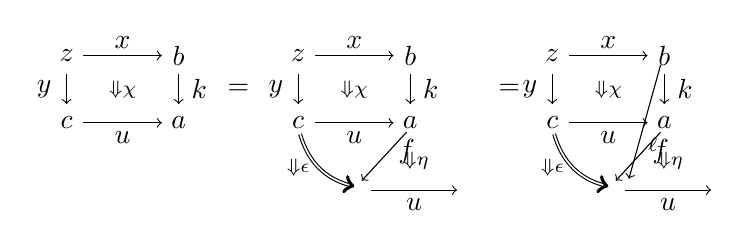
\begin{tikzpicture}[x=1.35em,y=1.35em]
  \node (z1) at (0,1.8) {$z$};
  \node (b1) at (3.0,1.8) {$b$};
  \node (c1) at (0,0) {$c$};
  \node (a1) at (3.0,0) {$a$};
  \draw[->] (0.45,1.8) -- (2.55,1.8);
  \node at (1.5,2.14) {$x$};
  \draw[->] (3.0,1.3) -- (3.0,0.5);
  \node at (3.55,0.9) {$k$};
  \draw[->] (0,1.3) -- (0,0.5);
  \node at (-0.6,0.9) {$y$};
  \draw[->] (0.45,0) -- (2.55,0);
  \node at (1.5,-0.4) {$u$};
  \node at (1.5,0.9) {$\scriptstyle\Downarrow\chi$};
  \node at (4.6,0.9) {$=$};
  \node (z2) at (6.2,1.8) {$z$};
  \node (b2) at (9.2,1.8) {$b$};
  \node (c2) at (6.2,0) {$c$};
  \node (a2) at (9.2,0) {$a$};
  \draw[->] (6.65,1.8) -- (8.75,1.8);
  \node at (7.7,2.14) {$x$};
  \draw[->] (9.2,1.3) -- (9.2,0.5);
  \node at (9.75,0.9) {$k$};
  \draw[->] (6.2,1.3) -- (6.2,0.5);
  \node at (5.6,0.9) {$y$};
  \draw[->] (6.65,0) -- (8.75,0);
  \node at (7.7,-0.4) {$u$};
  \node at (7.7,0.9) {$\scriptstyle\Downarrow\chi$};
  \draw[->] (9.1,-0.25) -- node[right,pos=0.4]{$f$} (7.9,-1.55);
  \node at (9.35,-1.0) {$\scriptstyle\Downarrow\eta$};
  \draw[->,double] (6.25,-0.3) to[bend right=30]
    node[left,pos=0.5]{$\scriptstyle\Downarrow\epsilon$} (7.7,-1.7);
  \draw[->] (8.15,-1.8) -- (10.45,-1.8);
  \node at (9.3,-2.2) {$u$};
  \node at (11.85,0.9) {$=$};
  \node (z3) at (13.0,1.8) {$z$};
  \node (b3) at (16.0,1.8) {$b$};
  \node (c3) at (13.0,0) {$c$};
  \node (a3) at (16.0,0) {$a$};
  \draw[->] (13.45,1.8) -- (15.55,1.8);
  \node at (14.5,2.14) {$x$};
  \draw[->] (16.0,1.3) -- (16.0,0.5);
  \node at (16.55,0.9) {$k$};
  \draw[->] (13.0,1.3) -- (13.0,0.5);
  \node at (12.4,0.9) {$y$};
  \draw[->] (13.45,0) -- (15.55,0);
  \node at (14.5,-0.4) {$u$};
  \node at (14.5,0.9) {$\scriptstyle\Downarrow\chi$};
  \draw[->] (15.9,-0.25) -- node[right,pos=0.4]{$f$} (14.7,-1.55);
  \node at (16.15,-1.0) {$\scriptstyle\Downarrow\eta$};
  \draw[->,double] (13.05,-0.3) to[bend right=30]
    node[left,pos=0.5]{$\scriptstyle\Downarrow\epsilon$} (14.5,-1.7);
  \draw[->] (14.95,-1.8) -- (17.25,-1.8);
  \node at (16.1,-2.2) {$u$};
  \draw[->] (15.9,1.55) -- node[right,pos=0.7]{$\scriptstyle\ell$} (15.05,-1.5);
\end{tikzpicture}
\end{center}
\begin{center}
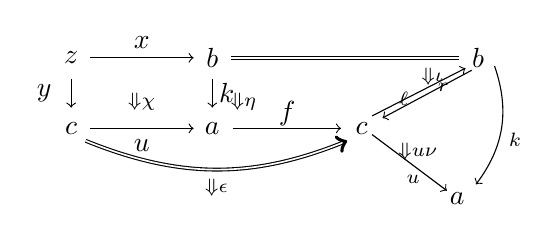
\begin{tikzpicture}[x=1.5em,y=1.5em]
  \node (z)  at (0,3.4)  {$z$};
  \node (b1) at (3.4,3.4) {$b$};
  \node (b2) at (9.8,3.4) {$b$};
  \draw[double] (3.85,3.4) -- (9.35,3.4);
  \node (c)  at (0,1.7)  {$c$};
  \node (a)  at (3.4,1.7) {$a$};
  \node (c2) at (7.0,1.7) {$c$};
  \node (a3) at (9.3,0)  {$a$};
  \draw[->] (0.45,3.4) -- (2.95,3.4);
  \node at (1.7,3.76) {$x$};
  \draw[->] (0,2.9) -- (0,2.2);
  \node at (-0.65,2.55) {$y$};
  \draw[->] (3.4,2.9) -- (3.4,2.2);
  \node at (3.75,2.55) {$k$};
  \draw[->] (0.45,1.7) -- (2.95,1.7);
  \node at (1.7,1.28) {$u$};
  \node at (1.7,2.35) {$\scriptstyle\Downarrow\chi$};
  \draw[->] (3.9,1.7) -- (6.5,1.7);
  \node at (5.2,2.06) {$f$};
  \node at (4.15,2.35) {$\scriptstyle\Downarrow\eta$};
  \draw[->,double] (0.35,1.4) to[bend right=22]
    node[below,pos=0.5]{$\scriptstyle\Downarrow\epsilon$} (6.65,1.4);
  \draw[->] (7.25,2.0) -- node[right,pos=0.6]{$\scriptstyle r$} (9.5,3.15);
  \draw[->] (9.65,3.1) -- node[left,pos=0.6]{$\scriptstyle\ell$} (7.5,1.95);
  \node at (8.7,2.95) {$\scriptstyle\Downarrow\iota$};
  \draw[->] (10.2,3.2) to[bend left=28] node[right,pos=0.6]{$\scriptstyle k$} (9.75,0.35);
  \draw[->] (7.25,1.55) -- node[below,pos=0.55]{$\scriptstyle u$} (9.05,0.2);
  \node at (8.35,1.15) {$\scriptstyle\Downarrow u\nu$};
\end{tikzpicture}
\end{center}

反之，若 $\zeta$ 给出 $\chi$ 经由 $u\nu$ 的一个分解，则
\begin{center}
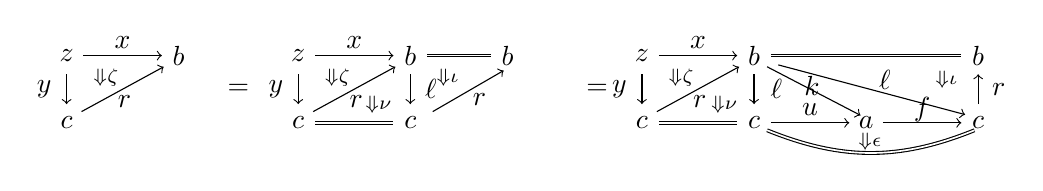
\begin{tikzpicture}[x=1.35em,y=1.35em]
  \node (z4) at (0,1.8) {$z$};
  \node (b4) at (3.0,1.8) {$b$};
  \node (c4) at (0,0) {$c$};
  \draw[->] (0.45,1.8) -- (2.55,1.8);
  \node at (1.5,2.14) {$x$};
  \draw[->] (0,1.3) -- (0,0.5);
  \node at (-0.6,0.9) {$y$};
  \draw[->] (0.4,0.3) -- (2.6,1.5);
  \node at (1.55,0.58) {$r$};
  \node at (1.05,1.22) {$\scriptstyle\Downarrow\zeta$};
  \node at (4.6,0.9) {$=$};
  \node (z5) at (6.2,1.8) {$z$};
  \node (b5) at (9.2,1.8) {$b$};
  \node (b6) at (11.8,1.8) {$b$};
  \draw[double] (9.65,1.8) -- (11.35,1.8);
  \node (c5) at (6.2,0) {$c$};
  \node (c6) at (9.2,0) {$c$};
  \draw[double] (6.65,0) -- (8.75,0);
  \draw[->] (6.65,1.8) -- (8.75,1.8);
  \node at (7.7,2.14) {$x$};
  \draw[->] (6.2,1.3) -- (6.2,0.5);
  \node at (5.6,0.9) {$y$};
  \draw[->] (6.6,0.3) -- (8.8,1.5);
  \node at (7.75,0.58) {$r$};
  \node at (7.25,1.22) {$\scriptstyle\Downarrow\zeta$};
  \node at (8.35,0.48) {$\scriptstyle\Downarrow\nu$};
  \draw[->] (9.2,1.3) -- (9.2,0.5);
  \node at (9.75,0.9) {$\ell$};
  \draw[->] (9.8,0.3) -- (11.7,1.4);
  \node at (11.05,0.62) {$r$};
  \node at (10.2,1.22) {$\scriptstyle\Downarrow\iota$};
  \node at (14.2,0.9) {$=$};
  \node (z6) at (15.4,1.8) {$z$};
  \node (b7) at (18.4,1.8) {$b$};
  \node (b8) at (24.4,1.8) {$b$};
  \draw[double] (18.85,1.8) -- (23.95,1.8);
  \node (c7) at (15.4,0) {$c$};
  \node (c8) at (18.4,0) {$c$};
  \node (a4) at (21.4,0) {$a$};
  \node (c9) at (24.4,0) {$c$};
  \draw[->] (15.85,1.8) -- (17.95,1.8);
  \node at (16.9,2.14) {$x$};
  \draw[->] (15.4,1.3) -- (15.4,0.5);
  \node at (14.8,0.9) {$y$};
  \draw[->] (15.8,0.3) -- (18.0,1.5);
  \node at (16.95,0.58) {$r$};
  \node at (16.45,1.22) {$\scriptstyle\Downarrow\zeta$};
  \node at (17.6,0.48) {$\scriptstyle\Downarrow\nu$};
  \draw[double] (15.85,0) -- (17.95,0);
  \draw[->] (18.4,1.3) -- (18.4,0.5);
  \node at (19.0,0.9) {$\ell$};
  \draw[->] (18.85,0) -- (20.95,0);
  \node at (19.9,0.36) {$u$};
  \draw[->] (21.85,0) -- (23.95,0);
  \node at (22.9,0.36) {$f$};
  \draw[->] (18.75,1.5) -- (21.25,0.2);
  \node at (19.95,0.98) {$k$};
  \draw[->] (19.05,1.55) -- (24.05,0.22);
  \node at (21.9,1.15) {$\ell$};
  \node at (23.55,1.15) {$\scriptstyle\Downarrow\iota$};
  \draw[->] (24.4,0.5) -- (24.4,1.3);
  \node at (24.95,0.9) {$r$};
  \draw[double] (18.75,-0.2) to[bend right=22] (24.3,-0.2);
  \node at (21.5,-0.5) {$\scriptstyle\Downarrow\epsilon$};
\end{tikzpicture}
\end{center}
\begin{center}
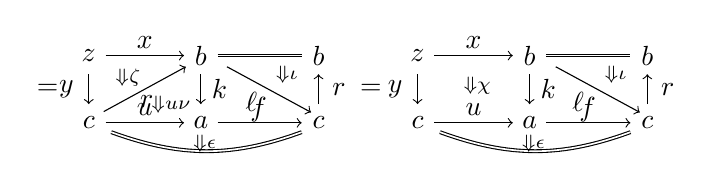
\begin{tikzpicture}[x=1.35em,y=1.35em]
  \node at (-1.1,0.9) {$=$};
  \node (z7) at (0,1.8) {$z$};
  \node (b9) at (3.0,1.8) {$b$};
  \node (b10) at (6.15,1.8) {$b$};
  \draw[double] (3.45,1.8) -- (5.7,1.8);
  \node (c10) at (0,0) {$c$};
  \node (a5) at (3.0,0) {$a$};
  \node (c11) at (6.15,0) {$c$};
  \draw[->] (0.45,1.8) -- (2.55,1.8);
  \node at (1.5,2.14) {$x$};
  \draw[->] (0,1.3) -- (0,0.5);
  \node at (-0.6,0.9) {$y$};
  \draw[->] (0.4,0.3) -- (2.6,1.5);
  \node at (1.55,0.58) {$r$};
  \node at (1.05,1.22) {$\scriptstyle\Downarrow\zeta$};
  \node at (2.2,0.48) {$\scriptstyle\Downarrow u\nu$};
  \draw[->] (3.0,1.3) -- (3.0,0.5);
  \node at (3.5,0.9) {$k$};
  \draw[->] (3.7,1.5) -- (5.95,0.28);
  \node at (4.35,0.55) {$\ell$};
  \node at (5.3,1.3) {$\scriptstyle\Downarrow\iota$};
  \draw[->] (6.15,0.5) -- (6.15,1.3);
  \node at (6.7,0.9) {$r$};
  \draw[->] (0.45,0) -- (2.55,0);
  \node at (1.5,0.36) {$u$};
  \draw[->] (3.45,0) -- (5.7,0);
  \node at (4.55,0.36) {$f$};
  \draw[double] (0.6,-0.25) to[bend right=20] (5.7,-0.25);
  \node at (3.1,-0.55) {$\scriptstyle\Downarrow\epsilon$};
  \node at (7.55,0.9) {$=$};
  \node (z8) at (8.8,1.8) {$z$};
  \node (b11) at (11.8,1.8) {$b$};
  \node (b12) at (14.95,1.8) {$b$};
  \draw[double] (12.25,1.8) -- (14.5,1.8);
  \node (c12) at (8.8,0) {$c$};
  \node (a6) at (11.8,0) {$a$};
  \node (c13) at (14.95,0) {$c$};
  \draw[->] (9.25,1.8) -- (11.35,1.8);
  \node at (10.3,2.14) {$x$};
  \draw[->] (8.8,1.3) -- (8.8,0.5);
  \node at (8.2,0.9) {$y$};
  \node at (10.4,1.0) {$\scriptstyle\Downarrow\chi$};
  \draw[->] (11.8,1.3) -- (11.8,0.5);
  \node at (12.3,0.9) {$k$};
  \draw[->] (12.5,1.5) -- (14.75,0.28);
  \node at (13.1,0.55) {$\ell$};
  \node at (14.1,1.3) {$\scriptstyle\Downarrow\iota$};
  \draw[->] (14.95,0.5) -- (14.95,1.3);
  \node at (15.5,0.9) {$r$};
  \draw[->] (9.25,0) -- (11.35,0);
  \node at (10.3,0.36) {$u$};
  \draw[->] (12.25,0) -- (14.5,0);
  \node at (13.35,0.36) {$f$};
  \draw[double] (9.4,-0.25) to[bend right=20] (14.5,-0.25);
  \node at (11.9,-0.55) {$\scriptstyle\Downarrow\epsilon$};
\end{tikzpicture}
\end{center}
这就证明了上文所构造的分解是唯一的。最后，由于绝对右\trLifting{}图的%
\trUniversalProperty{}由诸
伴随的存在所「以等式方式见证」，故它被任何\trTwoFunctor{}保持。
\end{proof}

\begin{example}\label{exa:delta-adjoint-diagram}
例如，存在由\trAdjunction{}\trFunctor{}构成的如下\trDiagram
\begin{center}
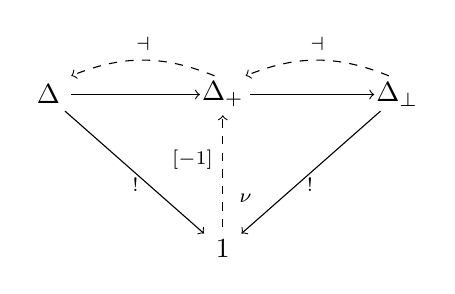
\begin{tikzpicture}[x=1.5em,y=1.5em]
  \node (D)  at (0,2.2)  {$\Delta$};
  \node (Dp) at (4.2,2.2) {$\Delta_{+}$};
  \node (Db) at (8.4,2.2) {$\Delta_{\perp}$};
  \draw[->] (0.55,2.2) -- (3.65,2.2);
  \draw[->] (4.85,2.2) -- (7.85,2.2);
  \draw[->,dashed] (4.0,2.65) to[bend right=22]
    node[above,pos=0.5]{$\scriptstyle\dashv$} (0.55,2.65);
  \draw[->,dashed] (8.2,2.65) to[bend right=22]
    node[above,pos=0.5]{$\scriptstyle\dashv$} (4.75,2.65);
  \node (one) at (4.2,-1.5) {$1$};
  \draw[->] (0.4,1.8) -- node[left,pos=0.6]{$\scriptstyle!$} (3.75,-1.15);
  \draw[->] (8.0,1.8) -- node[right,pos=0.6]{$\scriptstyle!$} (4.65,-1.15);
  \draw[->,dashed] (4.2,-1.0) -- node[left,pos=0.6]{$\scriptstyle[-1]$} (4.2,1.7);
  \node at (4.75,-0.3) {$\scriptstyle\nu$};
\end{tikzpicture}
\end{center}
它涉及第 2 章中的\cref{def:split-augmented}所引入的那些\trCategory{}。包含
$\Delta\hookrightarrow\Delta_{+}\hookrightarrow\Delta_{\perp}$ 自由地为每个序数
添入一个底元素，而其\trRightAdjoint{}则可等同于宽子范畴（其态射皆为保持底元素
的映射）的包含 $\Delta_{\perp}\hookrightarrow\Delta$。\trAdjunction{}
$[-1]\dashv\,!$ 见证
了下述事实：$[-1]\in\Delta_{\perp}$ 定义一个\trInitial{}对象，其\trCounit{} $\nu$
给出从该\trInitial{}对象到恒同\trFunctor{}的典范\trNaturalTransformation。这一%
\trDiagram{}在 $\Cat^{\mathrm{op}}$ 中满足\cref{lem:absolute-lifting-under-adjunction}的
前提。设 $a$ 为任一在 $\Cat$ 上\trCotensor{}的 2-\trCategory{} $\mathcal{C}$ 中的
一个对象，则 2-\trFunctor{} $a^{(-)}\colon\Cat^{\mathrm{op}}\to\mathcal{C}$ 把所给
数据携带为 $\mathcal{C}$ 中如下左图所示的\trAdjunction{}\trFunctor{}\trDiagram，从而如下右图所示
的三角形是一个绝对右\trLifting{}：
\begin{center}
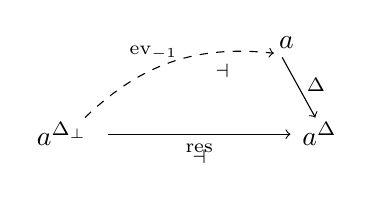
\begin{tikzpicture}[x=1.5em,y=1.5em]
  \node (aL)  at (5.4,2.2) {$a$};
  \node (aDbL) at (0,0) {$a^{\Delta_{\perp}}$};
  \node (aDL) at (6.2,0) {$a^{\Delta}$};
  \draw[->,dashed] (0.55,0.4) to[bend left=25]
    node[above,pos=0.4]{$\scriptstyle\mathrm{ev}_{-1}$}
    node[pos=0.68,below right]{$\scriptstyle\dashv$} (5.1,1.95);
  \draw[->] (5.3,1.85) -- node[right,pos=0.45]{$\scriptstyle\Delta$} (6.1,0.4);
  \draw[->] (1.1,0) -- node[below]{$\scriptstyle\mathrm{res}$} (5.5,0);
  \node at (3.3,-0.55) {$\scriptstyle\dashv$};
\end{tikzpicture}
\qquad
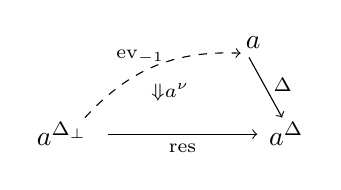
\begin{tikzpicture}[x=1.5em,y=1.5em]
  \node (aR)  at (4.6,2.2) {$a$};
  \node (aDbR) at (0,0) {$a^{\Delta_{\perp}}$};
  \node (aDR) at (5.4,0) {$a^{\Delta}$};
  \draw[->,dashed] (0.55,0.4) to[bend left=25]
    node[above,pos=0.4]{$\scriptstyle\mathrm{ev}_{-1}$} (4.3,1.95);
  \draw[->] (4.5,1.85) -- node[right,pos=0.45]{$\scriptstyle\Delta$} (5.3,0.4);
  \draw[->] (1.1,0) -- node[below]{$\scriptstyle\mathrm{res}$} (4.7,0);
  \node at (2.6,1.0) {$\scriptstyle\Downarrow a^{\nu}$};
\end{tikzpicture}
\end{center}
这就证明了第 2 章中的\cref{prop:split-limits}。
\end{example}

\begin{example}\label{exa:top-splitting-adjunctions}
存在一幅类似的由\trAdjunction{}\trFunctor{}构成的如下\trDiagram
\begin{center}
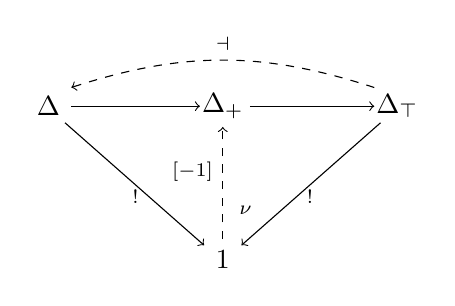
\begin{tikzpicture}[x=1.5em,y=1.5em]
  \node (D)  at (0,2.2)  {$\Delta$};
  \node (Dp) at (4.2,2.2) {$\Delta_{+}$};
  \node (Dt) at (8.4,2.2) {$\Delta_{\top}$};
  \draw[->] (0.55,2.2) -- (3.65,2.2);
  \draw[->] (4.85,2.2) -- (7.85,2.2);
  \draw[->,dashed] (7.85,2.65) to[bend right=18]
    node[above,pos=0.5]{$\scriptstyle\dashv$} (0.55,2.65);
  \node (one) at (4.2,-1.5) {$1$};
  \draw[->] (0.4,1.8) -- node[left,pos=0.6]{$\scriptstyle!$} (3.75,-1.15);
  \draw[->] (8.0,1.8) -- node[right,pos=0.6]{$\scriptstyle!$} (4.65,-1.15);
  \draw[->,dashed] (4.2,-1.0) -- node[left,pos=0.6]{$\scriptstyle[-1]$} (4.2,1.7);
  \node at (4.75,-0.3) {$\scriptstyle\nu$};
\end{tikzpicture}
\end{center}
它同样涉及第 2 章中的\cref{def:split-augmented}所引入的那些\trCategory{}。包含
$\Delta\hookrightarrow\Delta_{+}\hookrightarrow\Delta_{\top}$ 自由地添入一个顶元素，
而其\trRightAdjoint{}则可等同于宽子范畴（其态射皆为保持顶元素的映射）的包含
$\Delta_{\top}\hookrightarrow\Delta$。\trAdjunction{} $[-1]\dashv\,!$ 见证了下述
事实：$[-1]\in\Delta_{\top}$ 定义一个\trInitial{}对象，其\trCounit{} $\nu$
给出从该\trInitial{}对象到恒同\trFunctor{}的典范\trNaturalTransformation。这就
证明了第 2 章中的\cref{prop:split-limits}的另一个版本，其中「裂分」出现在
余／单纯对象的另一侧。
\end{example}

\begin{exercise}\label{ex:other-premise-diagrams}
试寻找由满足\cref{lem:absolute-lifting-under-adjunction}的前提的\trCategory{}构成的
其他\trDiagram，比如第 2 章中的\cref{ex:cospan-pullbacks}所隐含的那个例子。
\end{exercise}

